% !TeX program = pdflatex
% !TeX encoding = utf8
% !TeX spellcheck = russian_english
% !BIB program = biber


\IfFileExists{flags}{\input{flags}}{}
\documentclass{LabWorkEng}
\usepackage[type=none]{fgruler}
\addbibresource{\jobname.bib}


\newcolumntype{C}{>{\centering\arraybackslash}p{5em}}
\title{Study of rectilinear motion of bodies in the field of gravity using the Atwood machine}
\work{1}

\abstract{The purpose of this work is to test Newton's Second Law of Motion by utilizing an Atwood
	machine apparatus and determination of the acceleration of free fall in the field of gravity of the Earth. The Atwood machine will be used to study the relationship between mass, acceleration and net forces, with the distribution of the mass between the two weights being the independent variable and the time the dependent variable within the experiments.}



\keywords{Rectilinear motion of bodies, acceleration, free fall acceleration.}

\apparatus{Atwood machine consisting of one pulley with string attached over pulley to two
	weight hangers; sets of gram-weights, meter stick and stopwatch.}

\begin{document}
\writedatatofile{\jobname}
\maketitle

\nocite{IrodovMechanics, BerkeleyMechanics, FLF1, Holyday}
\printbibliography

\section{Theoretibal background}

The Atwood machine is designed to study the laws of motion of bodies in the field of gravity. Of course, it is best to study the field of gravity by exploring the free fall of bodies. But the acceleration of the Earth's gravity is quite large, and therefore the research must be carried out either at a very high device (height from the Pisa Tower), or by means of devices that allow measuring time with high accuracy (fractions of a second). The Atwood machine allows you to slow down the movement of the bodies at convenient speeds and using conventional devices to determine the acceleration of free fall.
\begin{figure}[!htbp]\centering
	\begin{subfigure}[b]{0.4\linewidth}\centering
		\begin{picbox}	
			\begin{tikzpicture}
			\tikzstyle{ground}=[fill,pattern=north east lines,draw=none,minimum width=0.75cm,minimum height=0.3cm]
			\node (wall1) [ground, minimum width=3cm] {};
			\draw (wall1.north west) -- (wall1.north east);
			\fill[gray!50] (-0.25,0.3) rectangle (0.25,10);
			\draw[ultra thick, fill=white] (0.0,10) circle (1);
			\draw[ultra thick] (0.0,10) circle (0.9);
			\draw[ultra thick] (-0.5,10) circle (0.3);
			\draw[ultra thick] (0.5,10) circle (0.3);
			\draw[ultra thick] (0,10.5) circle (0.3);
			\draw[ultra thick] (0,9.5) circle (0.3);
			\node[] at (-1.2,10) {$1$};
			\draw[fill=gray] (0.0,10) circle (0.1);
			\draw (-1,10) -- (-1,6);
			\fill[white, draw=black] (-1.5,6) node[left, text = black] {$m$} rectangle +(1,-0.1);
			\draw[thick, fill=gray] (-1.3,5.9) rectangle node[text = white] {A} +(0.6,-1);
			\draw (1,10) -- (1,4);
			\draw[thick, fill=gray] (0.7,4) rectangle node[text = white] {B} +(0.6,-1);
			\fill[gray, draw=black] (-1.5,8) node[left, text = black] {$2$} rectangle +(1.3,-0.1);
			\fill[gray, draw=black] (-1.5,4) node[left, text = black] {$3$} rectangle +(1.3,-0.1);
			\fill[gray, draw=black] (-1.5,2) node[left, text = black] {$4$} rectangle +(1.3,-0.1);
			\fill[gray!50, draw = black] (-1,0.3) rectangle +(2,1);
			\fill[red] (-0.9,1) rectangle +(0.3,0.1);
			\fill[black] (-0.9,0.8) rectangle +(0.3,0.1);
			\fill[black] (-0.9,0.6) rectangle +(0.3,0.1);
			\draw[fill=white] (-0.5,0.6) rectangle node[text = red] {time} +(1.3,0.5);
			\fill[black] (-0.9,0.15) rectangle +(0.3,0.15);
			\fill[black] (0.6,0.15) rectangle +(0.3,0.15);
			\node at (0.1,5) {\fgrulerdefnum{}\fgrulercaptioncm{}\ruler{upleft}{7cm}};
			\end{tikzpicture}
		\end{picbox}
		\subcaption{The Atwood machine.}
		\label{Atwood_machine}
	\end{subfigure}	
	\begin{subfigure}[b]{0.4\linewidth}\centering
		\begin{picbox}	
			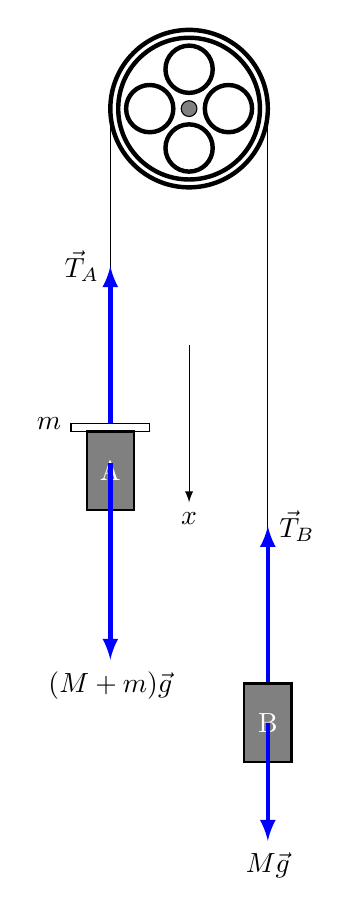
\begin{tikzpicture}
			\draw[ultra thick, fill=white] (0.0,10) circle (1);
			\draw[ultra thick] (0.0,10) circle (0.9);
			\draw[ultra thick] (-0.5,10) circle (0.3);
			\draw[ultra thick] (0.5,10) circle (0.3);
			\draw[ultra thick] (0,10.5) circle (0.3);
			\draw[ultra thick] (0,9.5) circle (0.3);
			\draw[fill=gray] (0.0,10) circle (0.1);
			\draw[-latex] (0,7) -- +(0,-2) node[below] {$x$};
			\draw (-1,10) -- (-1,6);
			\draw[-latex, ultra thick, blue] (-1,6) -- +(0,2) node[left, text = black] {$\vec{T}_A$};
			\fill[white, draw=black] (-1.5,6) node[left, text = black] {$m$} rectangle +(1,-0.1);
			\draw[thick, fill=gray] (-1.3,5.9) rectangle node[text = white] {A} +(0.6,-1);
			\draw[-latex, ultra thick, blue] (-1,5.5) -- +(0,-2.5) node[below, text = black] {$(M + m)\vec{g}$};
			\coordinate (B) at (1,2.7);
			\draw (1,10) --  (B);
			\draw[-latex, ultra thick, blue] (B) -- +(0,2) node[right, text = black] {$\vec{T}_B$};
			\draw[thick, fill=gray] ([shift={(-0.3,0)}]B) rectangle node[text = white] {B} +(0.6,-1);
			\draw[-latex, ultra thick, blue] ([yshift=-0.5cm]B) -- +(0,-1.5) node[below, text = black] {$M\vec{g}$};
			\end{tikzpicture}
		\end{picbox}
		\subcaption{Forces, acting on bodies.}
		\label{Forces}
	\end{subfigure}
	\caption{}
\end{figure}


The Atwood machine is depicted in Fig.~\ref{Atwood_machine}. Lightweight aluminum block 1 rotates freely around the horizontal axis, which is fixed to the top of the riser. A thin thread is thrown through the block, at the ends of which are weights A and B with equal masses $M$. If the body A loads a load of of $m$, then the balance weights will be broken and the system will begin to move with acceleration.

On the vertical column are fixed three consoles $2$, $3$, $4$. The console $2$ fixes the initial position of the body A. The body should be placed so that its the bottom edge was on one level with a white stripe on the console. On the consoles $3$ and $4$ there are two photo sensors, which allow to measure the time of fall of the body A.
At the beginning of the experiment, the load carrier A with the load was fixed thanks to the friction brake. Turning off the friction brake is released by the weight carrier and the system of weight workers begins to move equally quickly. When the body passes past the console $3$, the additional load is removed using a ring located on the same console, and then the system moves evenly. Thus, the photo-sensors capture the time of a uniform motion of the body-taker.


To determine the law of motion of body A, we choose a fixed reference system centered on the axis of the block. Take a look in more detail the forces acting on bodies A and B~(Fig.~\ref{Forces}). The $Ox$ axis is directed vertically down.

On the payload A there are two forces --- the gravity $(M + m)g$, and the force of the tension of the left part of the thread $T_A$. According to the second law of Newton:
\begin{equation}\label{1}
	\left( {M + m} \right)g - {T_A} = \left( {M + m} \right)a
\end{equation}
where $a$ -- acceleration of the body A.

Assuming that the thread combining the bodies does not stretch, the acceleration of the body B equals the absolute value of acceleration of the body A and is directed to the opposite side, that is, equals $-a$. Thus, for the body B, the second law of Newton has the form
\begin{equation}\label{2}
	Mg - T_A =  - Ma
\end{equation}
where $T_B$ -- tension force of the right (in the figure~\ref{Forces}) the end of the thread.

The relationship between the forces of tension $T_A$ and $T_B$ can be found from the equation of moments for the block, if you neglect the force of friction in the shafts of the axis of the block:

\begin{equation}\label{3}
	\left( {{T_A} - {T_B}} \right)r = \frac{{Ja}}{r}
\end{equation}
where $J$ -- moment of inertia of the block, $r$ -- its radius. From the equations \eqref{1} -- \eqref{2} we get the connection between the acceleration of free fall $g$ and the acceleration of the body $a$:


\begin{equation}\label{4}
	a = g\frac{m}{{2M + m + J/{r^2}}}
\end{equation}

Thus, the A carrier moves smoothly according to equation~\eqref{4}. If the weight of the load is much less than the mass of the masses $m \ll  M$ , then the acceleration a is much less than g, and therefore it is easier to measure. Formula~\eqref{4} is much simpler if we neglect the moment of block inertia:

\begin{equation}\label{5}
	a = g\frac{m}{{2M + m}}
\end{equation}


Using the formula~\eqref{4} or \eqref{5}, we can determine the acceleration of free fall. To do this, measure acceleration $a$. To determine $a$, we will use the fact that at the interval $h_1$ between the consoles $2$ and $3$ the gravity travels equally rapidly and acquires speed:

\begin{equation}\label{6}
	\upsilon  = \sqrt {2{h_1}a}
\end{equation}


After the carrier A is released from the load near the console $3$, it passes the distance $h_2$ between the consoles $3$ and $4$ at a constant velocity $v$. Measuring the time of a uniform motion $t$, we find
\begin{equation}\label{7}
	\upsilon  = \frac{{{h_2}}}{t}
\end{equation}
Comparing~\eqref{6} and~\eqref{7}, we finally calculate the acceleration:

\begin{equation}\label{8}
	a = \frac{{h_2^2}}{{2{h_1}{t^2}}}
\end{equation}


Deriving the formula~\eqref{8} we have neglected the force of air resistance.

\section{Experimental details}

The travel time of the weight is measured by an electronic stopwatch, which is retracted and disabled when the optical axis of the photosensors $3$ and $4$ passes, respectively. The stopwatch is ready for the next measurement only after pressing the  \tcbox{\sc{Reset}} button, which sets the stopwatch to zero.

In order for the system of heavy-duty loads to begin to move, it is necessary to press the \tcbox{\sc{Start}} button (with locking). In this case, the friction brake, which holds the weight in the initial position, is turned off;
the stopwatch comes to a standby state and starts when the photo dimension body is transmitted. After passing the photo sensor, the stopwatch switches off and the friction brake is activated.

The drop height is determined by the scale applied to the riser, by the difference in positions of the optical axes of the upper and lower photosensors. The weight of each of the weights and the mass of goods is determined experimentally. The measurement error of the consoles $2$, $3$, 4 is $\pm 1$~mm. The measurement error of time is determined experimentally. Instrumental measurement error of time -- $0.001$~seconds.

\section{Tasks}
Before starting systematic measurements, it is useful to do some experiments with different $h$ and $m$ to ensure that the installation is working properly.

\begin{enumerate}
	\item Determine the acceleration of the system of connected body with the load (Fig.~\ref{Atwood_machine}). Fix the console $3$. For selected $h_1$ and $h_2$ run a series of $10$ measurements of the time $t$ of the vehicle system between the $3$ and $4$ consoles. Is there enough data to determine $a$?
	\item Repeat the experiment for all available loads and their various combinations.
	\item Change the position of the console $3$ and repeat steps $2$ and $3$ for new values $h_1$ and $h_2$. Do this for the third pair $h_1$ and $h_2$.
	\item Weigh heavyweights of $m$ and $M$. Assess the value of $g$ from your data.
	\item Make the necessary measurements to estimate the moment of inertia of the dural unit $1$. Consider the sources of probable errors. Rate them. If you need experiments for this, make them.
\end{enumerate}

\section{Processing the results of the experiment}

\begin{enumerate}
	\item Average time $t$ for each experiment with a separate load $m$ and fixed $h_1$ and $h_2$. Determine the random error of time and compare with the error that the stopwatch inserts. Put the data in the table.
	\item For each case, using the formulas~\eqref{5} and \eqref{8}, calculate the acceleration $a$ and $g$. Identify the errors.
	\item Construct graphic dependence $g$ from $1/m$. What type is this relationship? Using the obtained dependence, determine the value of $g$. By which masses the resulting value is consistent with the best $g$ tabulated? %(See table~\ref{tab}).
	\item Evaluate the error of the experiment. Make conclusions.
\end{enumerate}

\section*{Control questions}
\begin{enumerate}[label*=\arabic*.]
	\item Formulate the basic kinematic quantities and explain their physical meaning.
	\item Write down the laws of velocity variation with time and the laws of motion in vector and coordinate forms for uniformly accelerated motion.
	\item Formulate the Newton's Laws.
	\item What is free fall? What is the acceleration of free fall $g$?
	\item Is the motion of the bodies in the work free fall?
	\item At what stage the motion of bodies is uniform (uniformly accelerated)?
	\item Apply Newton Second Law for the motion of bodies in work.
%	\item How else can measure the acceleration of gravity without using ultra-high and high-precision instruments?
%	\item Evaluate the required height of the device for direct study of the acceleration of free fall of bodies with the same accuracy as in this work in the Earth and on the surface of the Moon (the strength of the air resistance is neglected).
%	\item What are the disadvantages of indirect measurement methods?
%	\item How can photosensor be improved to reduce the delay in the operation of the photosensor?
	\item Why to determine $g$ we plot the dependence graph of $1/m$, but not of $m$?
	\item Is it possible to neglect the moment of inertia and friction? How do they affect the definition of $g$ for different loads? Is it possible somehow to prevent this effect when calculating $g$?
\end{enumerate}

%\begin{table}[!htbp]
%	\caption{Acceleration of gravity $g$ ($m/s^2$) at different latitude}
%	\label{tab}
%	\centering
%	\begin{tabular}{lcccccc}
%		\toprule
%		Latitude   & $0^\circ$ & $15^\circ$ & $30^\circ$ &         $45^\circ$          & $60^\circ$ & $75^\circ$ \\ \midrule
%		$0^\circ$  & $9.7803$  &  $9.7838$  &  $9.7932$  &          $9.8062$           &  $9.8191$  &  $9.8287$  \\
%		$1^\circ$  & $9.7803$  &  $9.7842$  &  $9.794$   &          $9.8071$           &  $9.8199$  &  $9.8291$  \\
%		$2^\circ$  & $9.7804$  &  $9.7847$  &  $9.7948$  &           $9.808$           &  $9.8207$  &  $9.8295$  \\
%		$3^\circ$  & $9.7804$  &  $9.7852$  &  $9.7956$  &          $9.8089$           &  $9.8214$  &  $9.8299$  \\
%		$4^\circ$  & $9.7806$  &  $9.7858$  &  $9.7965$  &          $9.8098$           &  $9.8222$  &  $9.8303$  \\
%		$5^\circ$  & $9.7807$  &  $9.7863$  &  $9.7973$  &          $9.8107$           &  $9.8229$  &  $9.8306$  \\
%		$6^\circ$  & $9.7809$  &  $9.7869$  &  $9.7982$  &          $9.8116$           &  $9.8236$  &  $9.8309$  \\
%		$7^\circ$  & $9.7811$  &  $9.7875$  &  $9.799$   & \cellcolor{red!25}$9.8124$ &  $9.8242$  &  $9.8312$  \\
%		$8^\circ$  & $9.7813$  &  $9.7882$  &  $9.7999$  &          $9.8133$           &  $9.8249$  &  $9.8314$  \\
%		$9^\circ$  & $9.7816$  &  $9.7888$  &  $9.8008$  &          $9.8142$           &  $9.8255$  &  $9.8316$  \\
%		$10^\circ$ & $9.7819$  &  $9.7895$  &  $9.8017$  &           $9.815$           &  $9.8261$  &  $9.8318$  \\
%		$11^\circ$ & $9.7822$  &  $9.7902$  &  $9.8026$  &          $9.8159$           &  $9.8266$  &  $9.8319$  \\
%		$12^\circ$ & $9.7825$  &  $9.7909$  &  $9.8035$  &          $9.8167$           &  $9.8272$  &  $9.832$   \\
%		$13^\circ$ & $9.7829$  &  $9.7917$  &  $9.8044$  &          $9.8175$           &  $9.8277$  &  $9.8321$  \\
%		$14^\circ$ & $9.7833$  &  $9.7924$  &  $9.8053$  &          $9.8184$           &  $9.8282$  &  $9.8321$  \\ \bottomrule
%	\end{tabular}%
%\end{table}

\end{document}